\newpage
\section{Datenverarbeitung}\label{sec:Datenverarbeitung}
Die Bewertung des Systemzustands erfolgt über die Ermittlung von drei zentralen Kennwerten. Zum einen muss der aktuelle Systemzustand ermittelt werden. Dieser ist eine Momentaufnahme, die innerhalb der letzten Minute erfasst wird. Er bildet das Kernelement der Bewertung. Alle weiteren Kennwerte bauen auf dem aktuellen Systemzustand auf. Im weiteren Verlauf wird dieser als \textit{SytemStatus} betitelt. Des Weiteren wird aus den Aufzeichnungen des \textit{SystesmStatus} der sogenannte \textit{HistorySystemStatus} ermittelt. Dieser liefert einen historischen Einblick in das Nutzungsverhalten des Systems über eine gewisse Zeit. Zuletzt kann über den \textit{HistorySystemStatus} die, in Abschnitt \ref{sec:MTBF} behandelte, Systemzuverlässigkeit errechnet werden.
\subsection{Health Status Definition}
\begin{wrapfigure}{r}{0.2\textwidth}
    \vspace{-1.2cm}
    \captionsetup{justification=centering,format=plain, font=small}
    \begin{center}
      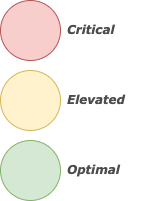
\includegraphics[width=0.2\textwidth]{HealthStatus.png}
    \end{center}
    \vspace{-0.5cm}
    \caption{}
    \label{fig:Systemstatus}
    \vspace{-0.5cm}
\end{wrapfigure}
Der Betrieb der Zielplattform wird zunächst in drei Zustände unterteilt. Sind alle Temperatur und die CPU Auslastung in der Norm, so läuft die Plattform im \textit{Optimal} Bereich. Steigen Temperaturen oder CPU Auslastung, so steigt der Status auf \textit{Elevated}. Erreicht die Temperatur nun Grenzwerte, die nicht überschritten werden dürfen, begibt sich der SystemStatus in den \textit{Critical} Bereich.\\
Der \textit{Systemstatus} wird daher in die drei Zustände \textit{Optimal}, \textit{Elevated} und \textit{Critical} unterteilt. Der SystemStatus wird, wie in  Abbildung \ref{fig:Systemstatus}, nach dem Ampelprinzip visualisiert.\\
Die Algorithmen zur Ermittlung dieser Werte sind unabhängig von der Hardwarekonfiguration der verschiedenen Zielplattformen. Lediglich die verwendeten Daten, die den Algorithmen zur Verfügung gestellt werden, unterscheiden sich für jede Plattform. In den folgenden Abschnitten werden die Algorithmen auf die VisuNet FLX Plattform ausgelegt. Dabei wird die Architektur so ausgelegt, dass sie für alle anderen Plattformen verwendet werden kann.
\newpage
\subsubsection*{Hardwarekonfiguration der VisuNet FLX Platform}\label{sec:FLXHardwarekonfiguration}
\begin{wrapfigure}{r}{0.3\textwidth}
    \vspace{-1.2cm}
    \captionsetup{justification=centering,format=plain, font=small}
    \begin{center}
        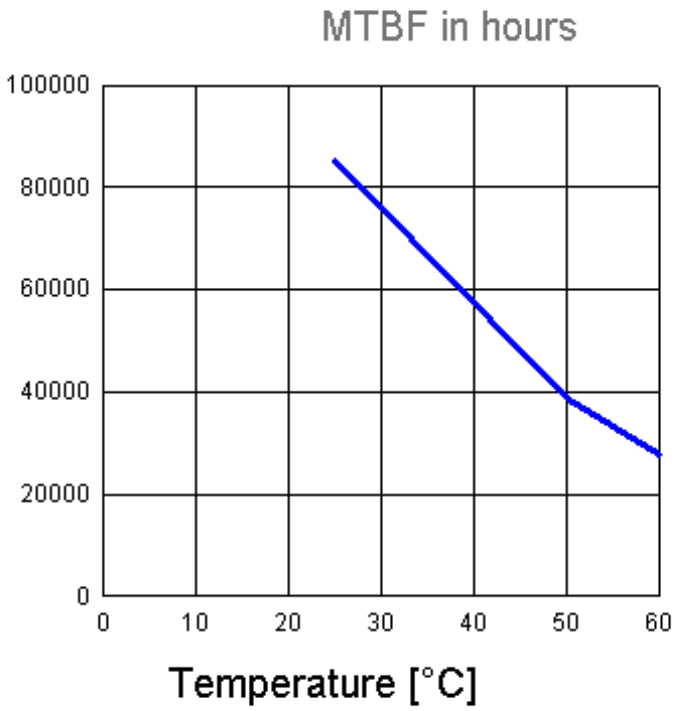
\includegraphics[width=0.3\textwidth]{FLXMTBFPrediction}
    \end{center}
    \vspace{-0.5cm}
    \caption{\ac{mtbf} Vorhersage für die VisuNet FLX Plattform}
    \label{fig:FLXMTBF}
    \vspace{-0.5cm}
\end{wrapfigure}
Damit die Ergebnisse der Bewertungsalgorithmen möglichst genau sind, ist es wichtig, mit den richtigen Werten zu rechnen. Zum einen müssen daher die richtigen Temperaturgrenzen für das System festgelegt werden.\\
Die aus Anhang \ref{app:mtbfprediction} entnommene Abbildung \ref{fig:FLXMTBF} stellt den \ac{mtbf}, der VisuNet FLX Plattform, in Abhängigkeit zur Betriebstemperatur des Gerätes dar. Aus dieser werden drei Intervalle für den Betrieb des Gerätes festgelegt. Von 0°C bis 45°C läuft das Gerät im \textit{Optimal} Betrieb. Dabei wird für dieses Intervall eine \ac{mtbf} von 60000h angenommen. Im zweiten Intervall von 45°C bis 63°C läuft das Gerät im \textit{Elevated} Betrieb. Der angenommene \ac{mtbf} für dieses Intervall ist 40000h. Bei allem über 63°C läuft das Gerät im \textit{Critical} betrieb, mit einem \ac{mtbf} 30000h.\\
\vspace{-1cm}
\begin{center}
    \begin{figure}[h!]
        \centering
        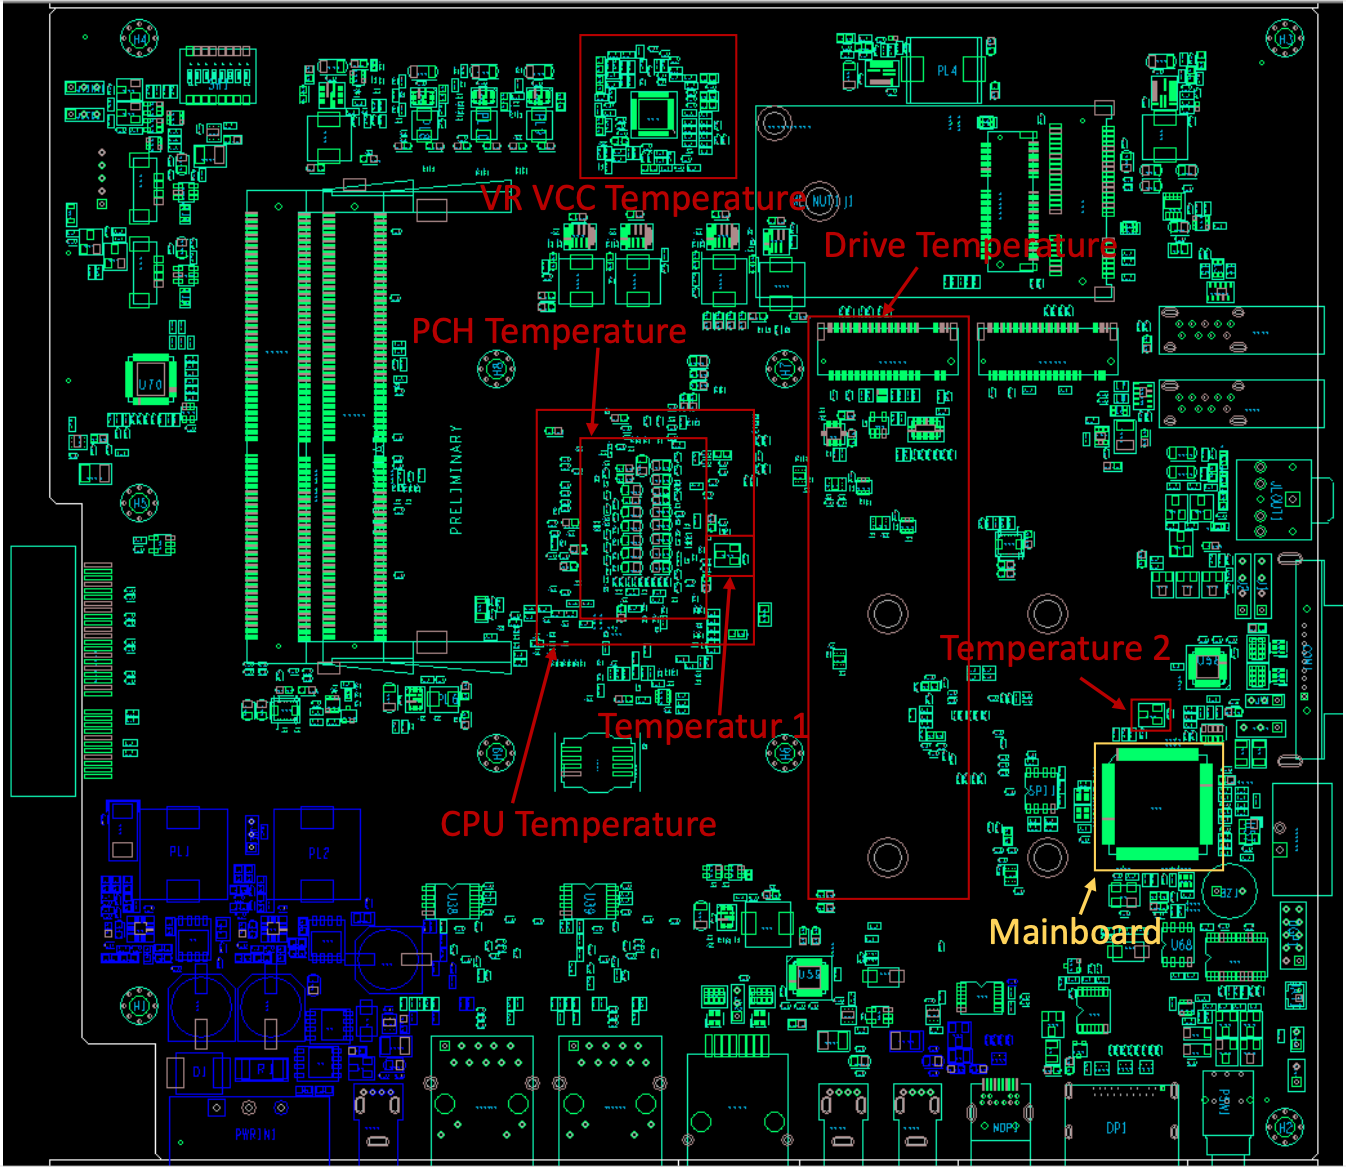
\includegraphics[width=0.8\textwidth]{FLXSensorPlatzierung}
        \caption{Sensorverteilung auf der Mainboard Platine der VisuNet FLX Plattform}
        \label{fig:FLXSensoren}
    \end{figure}
\end{center}
\vspace{-2.5cm}
Um die \ac{mtbf} Vorhersage aus Abbildung \ref{fig:FLXMTBF} mit den Temperaturen der Hardware verwenden zu können, müssen hierfür die richtigen Sensoren verwendet werden. Abbildung \ref{fig:FLXSensoren} zeigt die Sensorverteilung auf der VisuNet FLX Plattform. Da CPU und Spannungsregulator (siehe Abb. \ref{fig:FLXSensoren} \textit{VR VCC Temperature} und \textit{CPU Temperature}) zwei signifikante Hitzequellen sind, wird der Sensor \textit{Temperatur 1} zur Bestimmung der Betriebstemperatur gewählt. 
\vspace{-0.5cm}
\subsection{Auslegung einer Fuzzy Logik zur Ermittlung des Systemstatus}\label{sec:SystemStatusErmittelung}
Der \textit{SystemStatus} wird mithilfe des, in Abschnitt \ref{sec:FuzzyLogic} beschriebenen, Fuzzy-Logic Verfahren ermittelt. Das System soll dabei so ausgelegt werden, dass der \textit{SystemStatus} von Temperatur und CPU-Last abhängt.\\
Im ersten Schritt müssen daher zunächst die linguistischen Variablen, welche die Ein- und Ausgänge der Fuzzyengine repräsentieren, definiert werden. Zudem müssen auch die passenden Zugehörigkeitsfunktionen der Ein- und Ausgänge definiert werden. Diese sind mathematische Funktionen, welche angeben, wie stark ein Wert zu einem bestimmten linguistischen Begriff gehört. \cite{FuzzyLogicGeeks}\\ 
\vspace{-1.5cm}
\subsubsection*{Definition der linguistischen Variablen und der Zugehörigkeitsfunktionen}
\vspace{-0.5cm}
Die Temperaturen werden der linguistischen Variable \textit{Temperature} zugeordnet. Zudem werden drei Zugehörigkeitsfunktionen definiert. Diese sind in Abbildung \ref{fig:MSFTemp} abgebildet. Dabei werden die Grenzen der Funktionen an die in Abschnitt \ref{sec:FLXHardwarekonfiguration} aufgestellten Temperaturintervalle angepasst. Es werden insgesamt drei trapezförmige Funktionen erstellt. Die Funktionen werden mit den Begriffen \textit{Low}, \textit{Medium} und \textit{High} bezeichnet.
\vspace{-0.4cm}
\begin{center}
    \begin{figure}[h!]
        \captionsetup{justification=centering,format=plain, font=small}
        \centering
        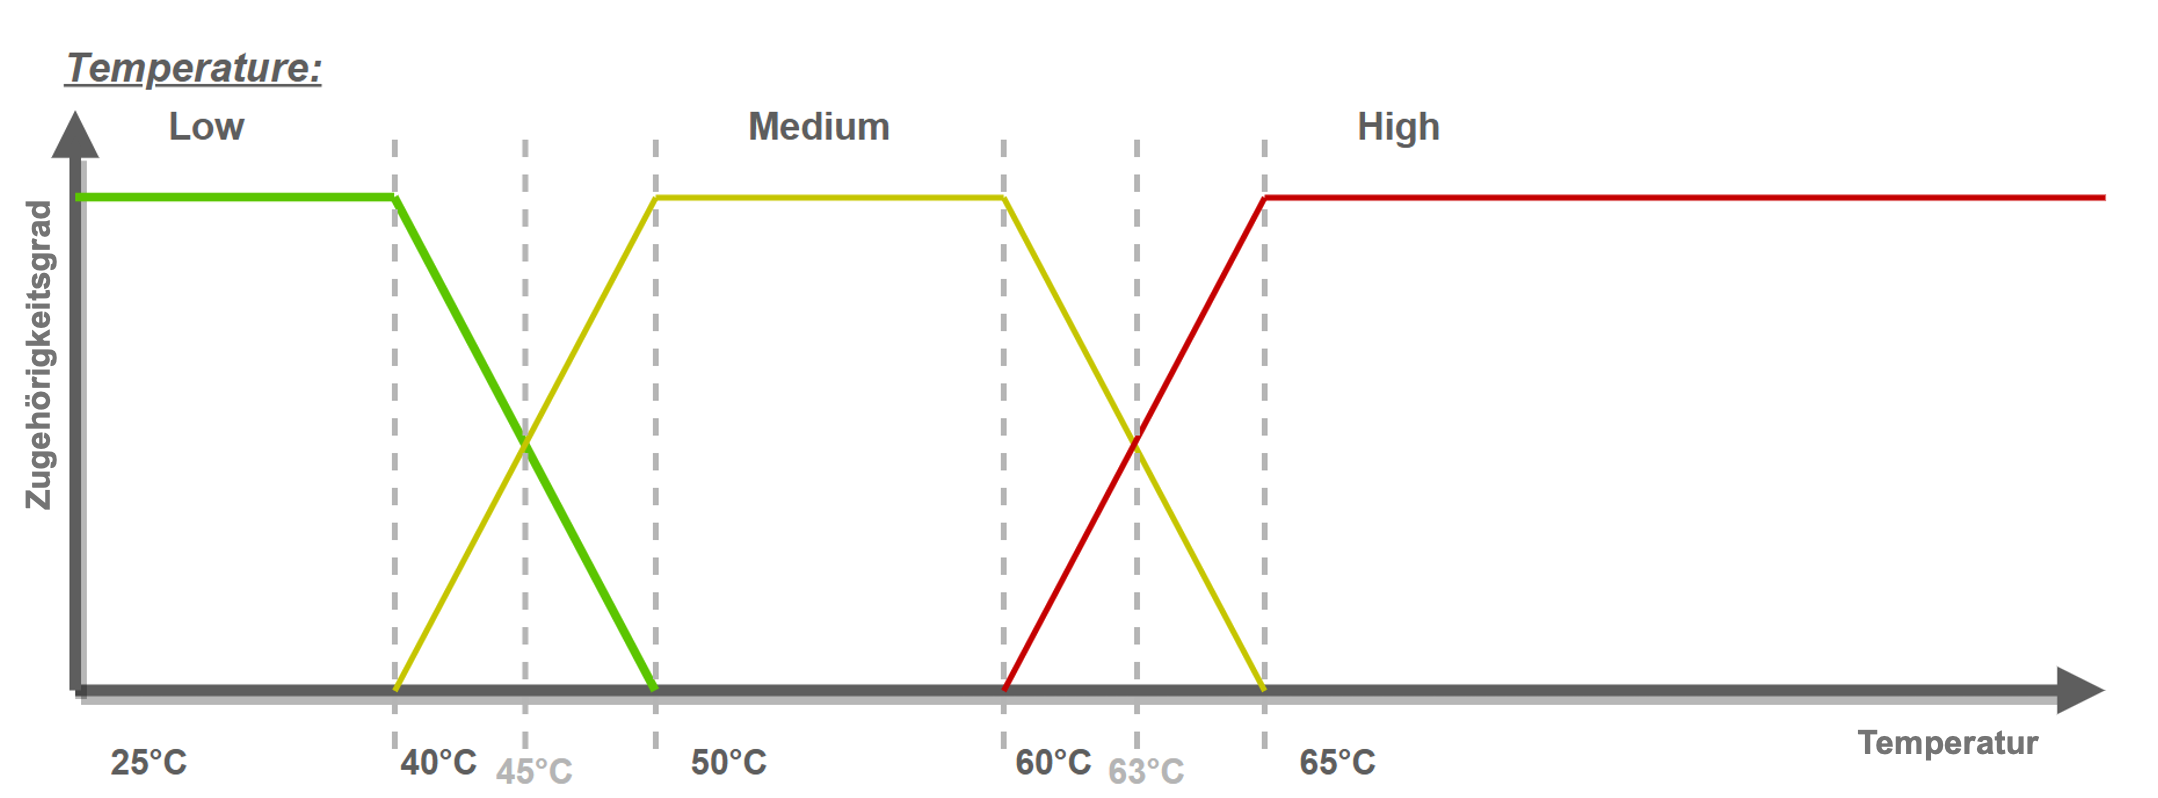
\includegraphics[width=0.9\textwidth]{MSFTemp.png}
        \caption{Zugehörigkeitsfunktionen der Temperature Variable}
        \label{fig:MSFTemp}
    \end{figure}
\end{center}
\vspace{-0.5cm}
Die Auslastung der CPU wird der linguistischen Variable \textit{CPULoad} zugeordnet. Wie auch bei den Zugehörigkeitsfunktionen der Temperatur werden hierfür ebenfalls drei trapezförmige Funktionen aufgestellt. Diese werden ebenfalls mit den Begriffen \textit{Low}, \textit{Medium} und \textit{High} bezeichnet. Die Zugehörigkeitsfunktionen der Variable \textit{CPULoad} werden in Abbildung \ref{fig:MSFCPULoad} dargestellt.
\begin{center}
    \begin{figure}[h!]
        \captionsetup{justification=centering,format=plain, font=small}
        \centering
        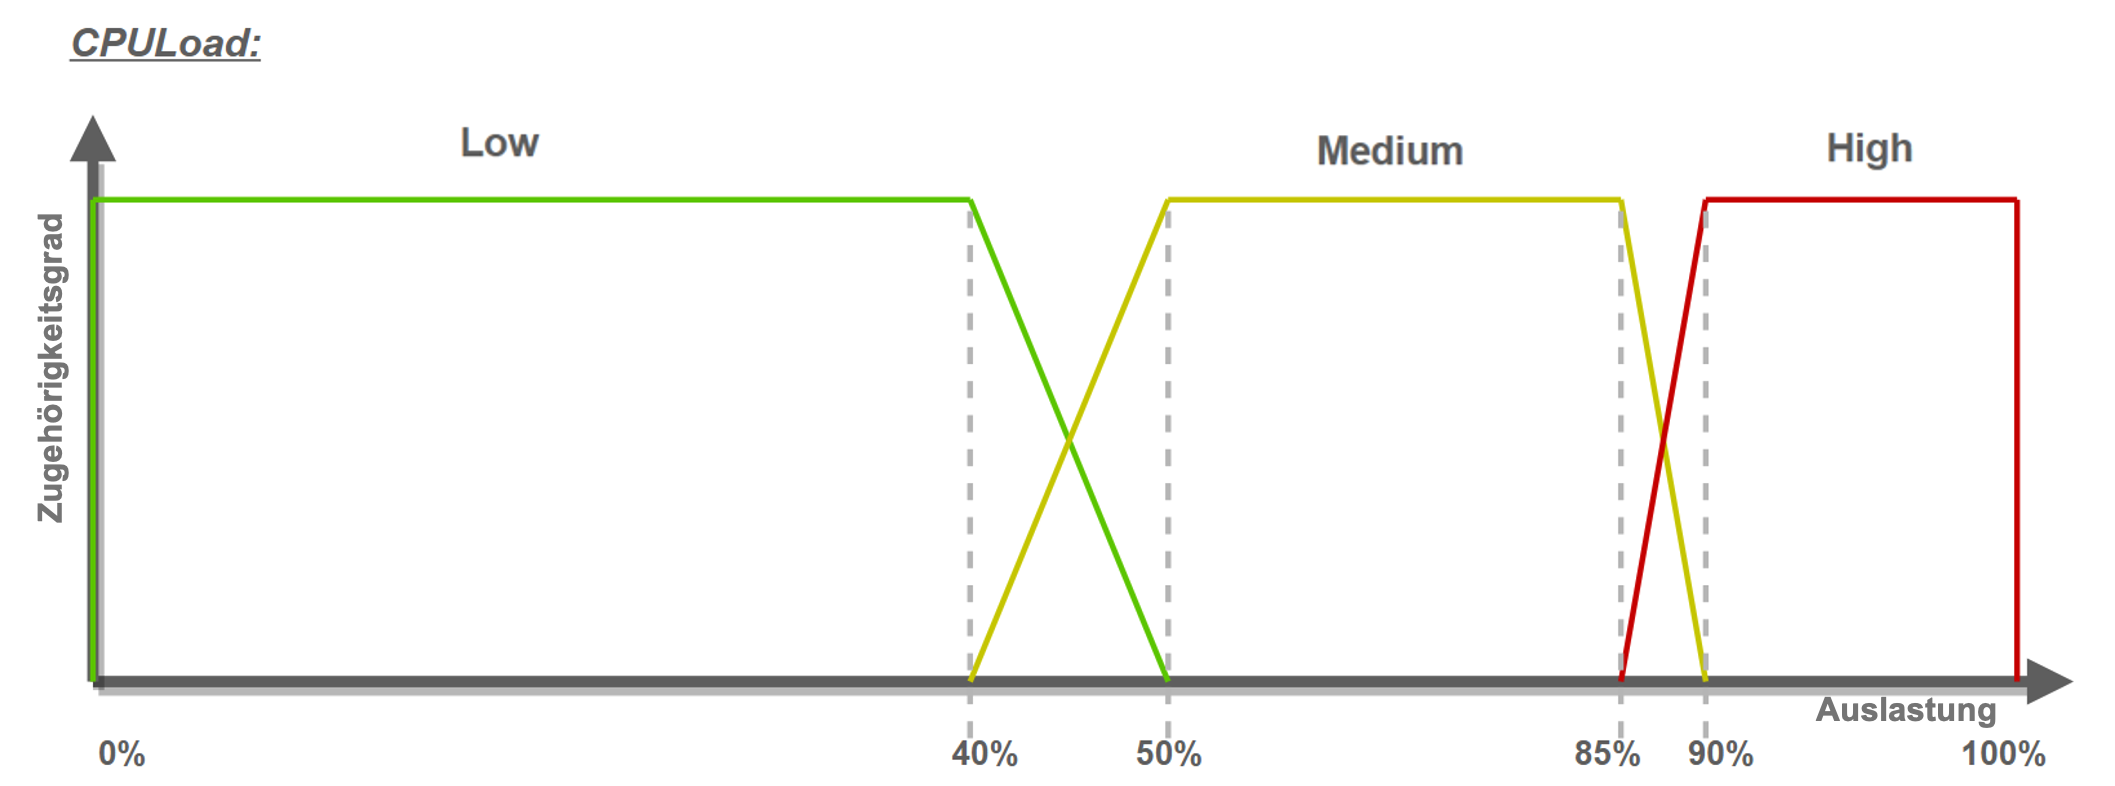
\includegraphics[width=0.9\textwidth]{MSFCPULoad.png}
        \caption{Zugehörigkeitsfunktionen der CPULast Variable}
        \label{fig:MSFCPULoad}
    \end{figure}
\end{center}
\vspace{-0.5cm}
Der Ausgang der Engine wird als die linguistische Variable \textit{SystemStatus} deklariert. Hierzu werden drei Rechteckfunktionen \textit{Optimal}, \textit{Elevated} und \textit{Critial} erzeugt. Das Ergebnis wird in \% angegeben, wobei jede Funktion genau ein Drittel darstellt. Die Funktionen der \textit{SystemStaus} Variable sind in Abbildung \ref{fig:MSFSystemStaus} dargestellt.
\begin{center}
    \begin{figure}[h!]
        \captionsetup{justification=centering,format=plain, font=small}
        \centering
        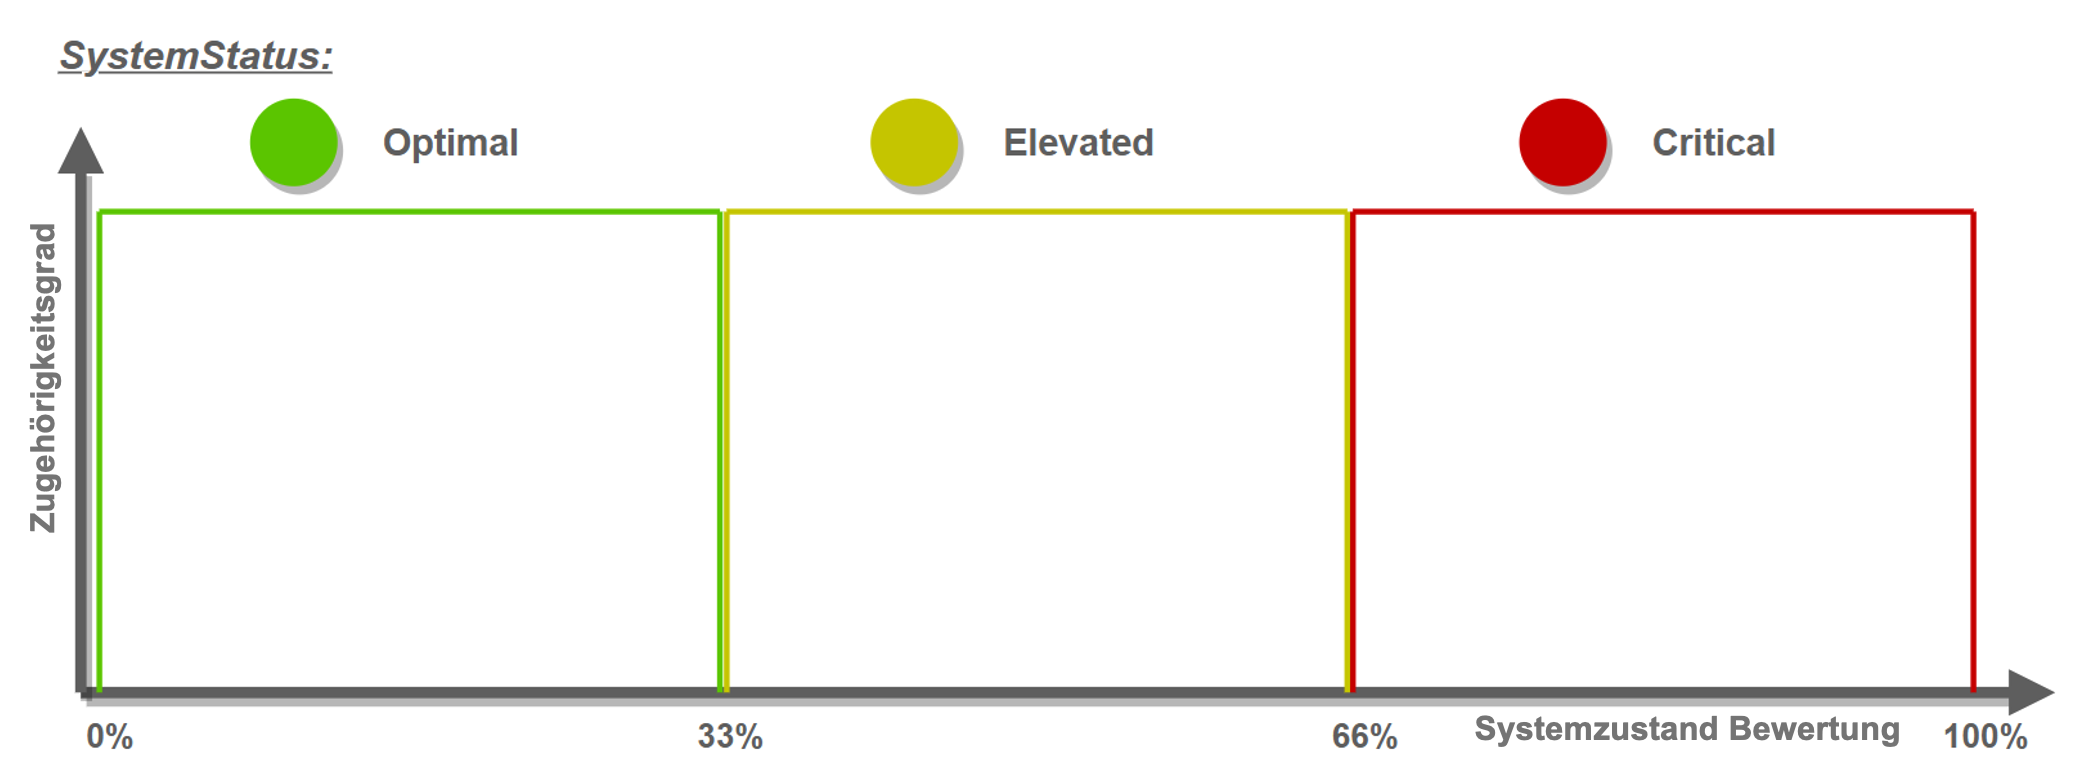
\includegraphics[width=0.9\textwidth]{MSFSystemStaus.png}
        \caption{Zugehörigkeitsfunktionen der SystemStatus Variable}
        \label{fig:MSFSystemStaus}
    \end{figure}
\end{center}
\vspace{-0.5cm}  

\subsubsection*{Definition der Regeln}\label{sec:FLRuleBase}
Im zweiten Schritt beim Auslegen eines Fuzzy-Logic Systems muss das Regelwerk festgelegt werden. Die Regeln eines solchen Systems sind dabei verbal gefasst und drücken die Beziehung zwischen den linguistischen Variablen der Ein- und Ausgänge aus.\cite{FLRegelwerk} \\
Die Ausgangsvariablen \textit{SystemStatus} wird in Abhängigkeit von den Eingangsvariablen \textit{Temperature} und \textit{CPLoad} gesetzt. Dabei werden die möglichen Zustände der Variable, die in Abbildung \ref{fig:MSFSystemStaus} gezeigt werden, wie folgt definiert. 
\begin{enumerate}
    \item \textit{SystemStatus: Optimal}\\
    Das System operiert im \textit{Optimal} Bereich, solange die Temperatur des Systems in den Wertebereich der Zugehörigkeitsfunktion \textit{Low} fällt. Zudem muss die Auslastung der CPU den Wertebereich der Zugehörigkeitsfunktionen \textit{Low} oder \textit{Medium} liefern.  
    \item \textit{SystemStatus: Elevated}\\
    Das System operiert im \textit{Elevated} bereich, sobald die Temperatur des Systems in den Wertebereich der Zugehörigkeitsfunktion \textit{Medium} oder die Auslastung der CPU in den Wertebereich der Zugehörigkeitsfunktion \textit{High} fällt.
    \item \textit{SystemStatus: Critical}\\
    Das System operiert im \textit{Critical} bereich, wenn die Temperatur des Systems in den Wertebereich der Zugehörigkeitsfunktion \textit{High} fällt. Dies bleibt unabhängig von der CPU Auslastung des Systems. 
\end{enumerate}
Aus dieser Zustandsdefinition kann somit das, in Abschnitt \ref{fig:FuzzyLogicRuleBase} gezeigte, Regelwerk zur Ermittlung des Systemzustands abgeleitet werden.  
\begin{center}
    \begin{figure}[h!]
        \captionsetup{justification=centering,format=plain, font=small}
        \centering
        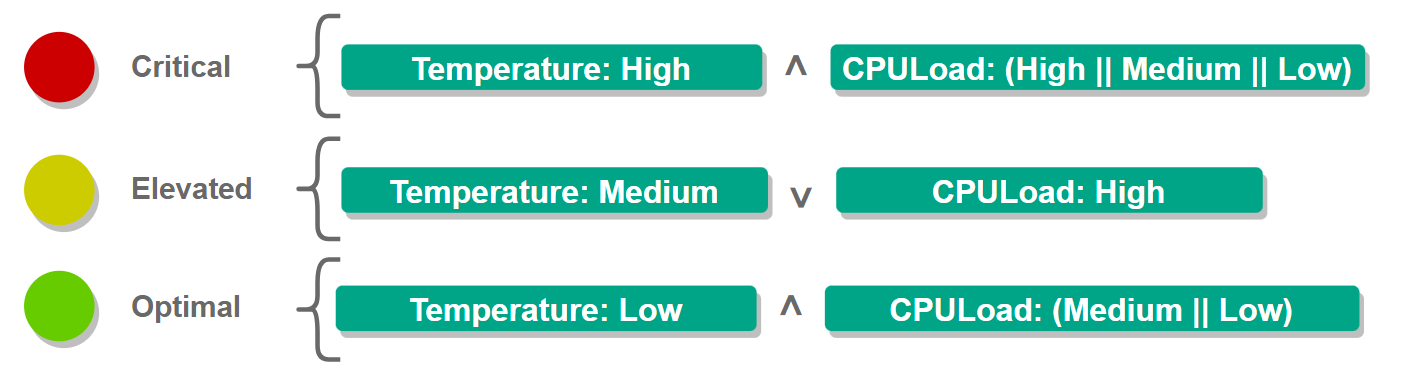
\includegraphics[width=1\textwidth]{RegelWerk.png}
        \caption{Regelwerk zum Ermitteln des Systemstauts}
        \label{fig:FuzzyLogicRuleBase}
    \end{figure}
\end{center}
\vspace{-0.5cm}  

\subsubsection*{Architektur}
Da die Basis der FuzzyLogic für jede Zielplattform dieselbe ist, wird zunächst über das \textit{IFuzzyLogic} Interface, die Schnittstelle zur Fuzzy Engin definiert. Hier raus wird anschließend die abstrakte Basisklasse \textit{FuzzyLogic} abgeleitet. Diese beinhaltet die verwendeten linguistischen Variablen, die jeweiligen Zugehörigkeitsfunktionen, so wie die Methoden zur Berechnung der Ergebnisse.\\
Aus der \textit{FuzzyLogic} Klasse können anschließend weitere Klassen abgeleitet werden, in denen die gewünschten Zugehörigkeitsfunktionen für die jeweiligen Zielplattformen angelegt werden können. Das in der Basisklasse definierte Regelwerk kann bei Bedarf in der abgeleiteten Klasse überschrieben werden. Die Struktur des \textit{HM.ScoringModel} Verzeichnisses wird in Abbildung \ref{fig:ScoringModel} visualisiert.  
\begin{center}
    \begin{figure}[h!]
        \captionsetup{justification=centering,format=plain, font=small}
        \centering
        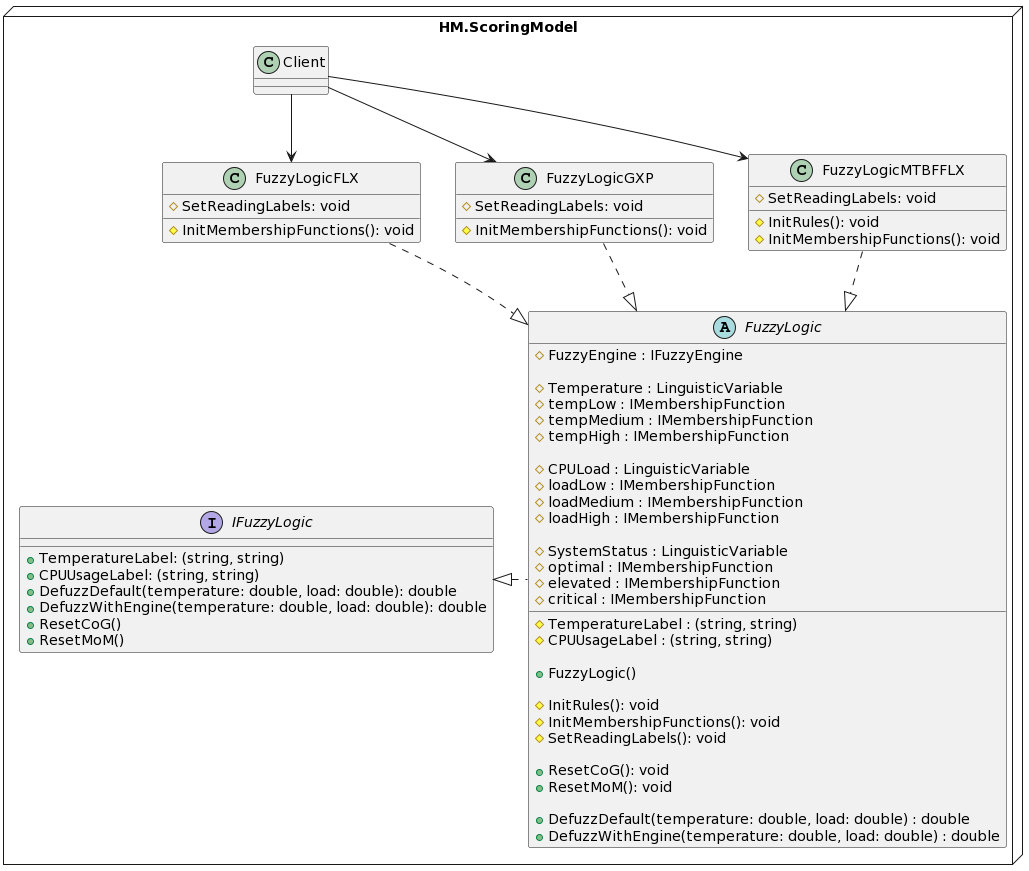
\includegraphics[width=1\textwidth]{ScoringModel.png}
        \caption{Architektur des HM.ScoringModel für die Ermittelung des SystemStatus}
        \label{fig:ScoringModel}
    \end{figure}
\end{center}

\subsection{Ermittlung der Systemstatus Historie und der Systemzuverlässigkeit}\label{sec:SystemHistoryReliability}
Um die Systemstatus Historie zu berechnen, werden die Aufzeichnungen des Systemstatus benötigt. Diese müssen im gewünschten Intervall, beispielsweise der letzten 24h, gegeben sein.
Die Idee besteht im Wesentlichen daraus, die Zeit zwischen zwei Systemzuständen, für jeden Zustand zu addieren. Somit kommt man auf die Zeiten, die das System im jeweiligen Zustand verbracht hat. Anschließend können die einzelnen Zeiten durch die gesamte Zeit des Intervalls geteilt werden, um auf die prozentualen Anteile der jeweiligen Zustände zu kommen.\\
Hierzu visualisiert das in Abbildung \ref{fig:SystemStatusHistoryAlgorythmus} visualisierte Ablaufdiagramm, die Ermittlung der Systemstatus Historie. Die Systemstatus Historie wird in der \textit{HistorySystemStatus} Tabelle der Datenbank abgespeichert. (Siehe Abbildung \ref{fig:DBModellErweitert})
\begin{center}
    \begin{figure}[h!]
        \captionsetup{justification=centering,format=plain, font=small}
        \centering
        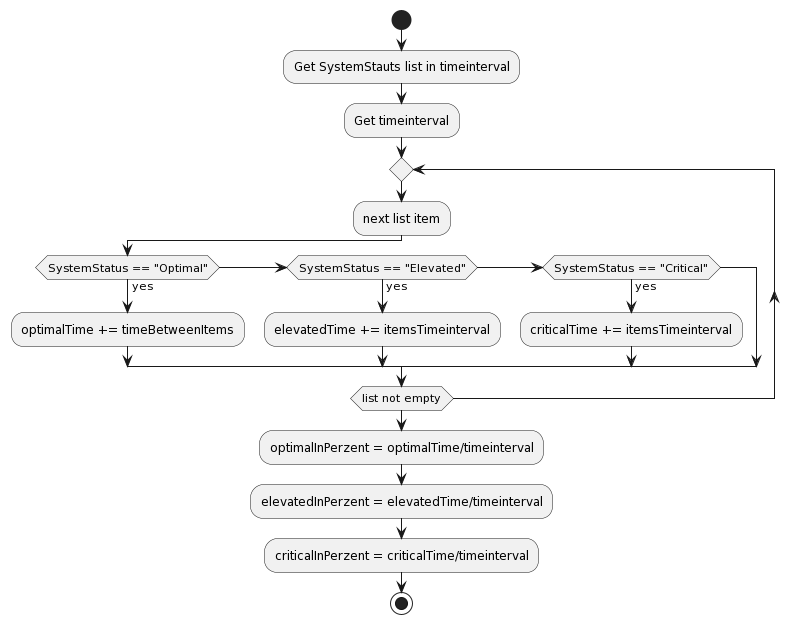
\includegraphics[width=0.87 \textwidth]{SystemStatusHistory.png}
        \caption{Algorithmus zur Berechnung der Systemstatus Historie}
        \label{fig:SystemStatusHistoryAlgorythmus}
    \end{figure}
\end{center}
\vspace{-1cm}
Über die in Abschnitt \ref{sec:MTBF} beschriebe Formel \ref{equ:Reliability} kann die  Reliability (Zuverlässigkeit) des Systems berechnet werden. Hierzu wird zum einen die Laufzeit des Systems, zum anderen der temperaturabhängige \ac{mtbf} des Systems benötigt. Jedoch kann diese Formel nicht direkt angewendet werden. Zum einen gibt es keine direkte Aufzeichnung über die gesamte Laufzeit des Systems. Zum anderen variiert die Betriebstemperatur des Systems, sodass man für verschiedene Betriebstemperaturen verschiedene \ac{mtbf} Werte verwenden muss.\\
Abhilfe hierzu schaft der Algorithmus zur Kalkulation der Systemstatus Historie. Die Idee hinter diesem Ansatz besteht darin, die unterschiedlichen Betriebstemperaturen mithilfe der \textit{FuzzyLogic} Klasse und einem angepassten Regelwerk aufzuzeichnen. Anschließend kann hierzu die Systemstatus Historie berechnet werden. Das Ergebnis liefert somit eine genaue Aussage darüber, wie lange das System in welchem Temperaturbereich gearbeitet hat. Somit bekommt man zum einen die Systemlaufzeit, zum anderen den zugehörigen temperaturabhängigen \ac{mtbf} zur Berechnung der Systemzuverlässigkeit.\\ 
Um bei der Berechnung der Systemzuverlässigkeit nicht jedes Mal alle Werten zu benutzen, wird diese zudem nur für eine kleine Zeitspanne, beispielsweise alle 24h, erneut durchgeführt. Das Ergebnis kann anschließend mit dem Ergebnis der vorherigen Berechnung verrechnet werden, um auf die aktuelle Systemzuverlässigkeit zu kommen.\\
Um die Berechnung durchführen zu können, muss daher zunächst das Regelwerk der FuzzyEngin angepasst werden. Hierzu wird die in Abbildung \ref{fig:FuzzyLogicArchitektur} abgebildete Klasse \textit{FuzzyLogicMTBFFLX} mit dem in Abbildung \ref{fig:SystemMTBF} abgebildeten Regelwerk angelegt. Der Ausgang \textit{SystemStatus}, der Eingang \textit{Temperature}, sowie die korrespondierenden Zugehörigkeitsfunktionen bleiben dabei unverändert. (Siehe Abbildung \ref{fig:MSFSystemStaus} und \ref{fig:MSFTemp}). Eingang \textit{CPULoad} fällt weg. Der Zustand des Eingangs wird eins zu eins auf den Ausgang übersetzt. Abbildung \ref{fig:SystemMTBF} veranschaulicht das angepasste Regelwerk der \textit{SuzzyLogicMTBFFLX} Klasse.
\begin{center}
    \begin{figure}[h!]
        \captionsetup{justification=centering,format=plain, font=small}
        \centering
        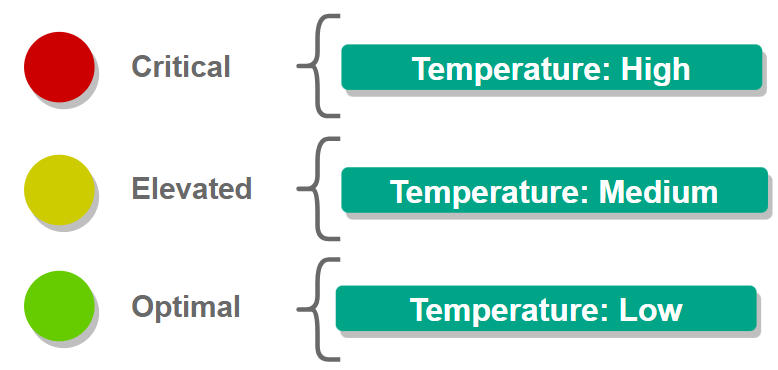
\includegraphics[width=0.6\textwidth]{RegelWerkMTBF.png}
        \caption{Regelwerk SystemMTBF}
        \label{fig:SystemMTBF}
    \end{figure}
\end{center}
\vspace{-0.5cm}
Das zuvor beschriebene Verfahren zur Ermittlung der Systemzuverlässigkeit wird in Abbildung \ref{fig:AblaufdiagramSystemReliability} visualisiert.
\begin{center}
    \begin{figure}[h!]
        \captionsetup{justification=centering,format=plain, font=small}
        \centering
        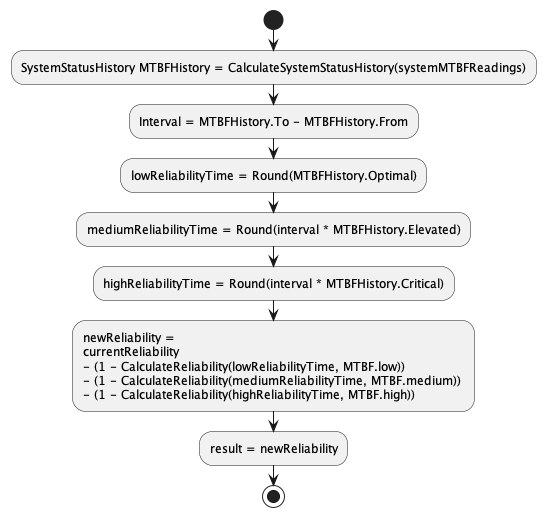
\includegraphics[width=0.7\textwidth]{SystemReliabilityBerechnung.png}
        \caption{Algorithmus zur Berechnung der Systemzuverlässigkeit}
        \label{fig:AblaufdiagramSystemReliability}
    \end{figure}
\end{center}

\subsubsection*{Klassenarchitektur}
Da die Algorithmen zum Berechnen der Systemstatus Historie so wie der Reliability des Systems unabhängig von Hardwarekonfiguration sind, wird das Verzeichnis \textit{HM.ScoringModel} um die, in Abbildung \ref{fig:SystemHistoryWrapper} abgebildete \textit{StatusHistory} Klasse erweitert. Diese bietet zwei Funktionen, mit welchen die Systemzuverlässigkeit so wie die Systemstatus Historie berechnet werden können. Da lediglich die temperaturabhängigen \ac{mtbf} Werte der Zielplattformen sich unterscheiden können, sollen diese beim Aufruf der Funktion \textit{CalculateCurrentReliability()} übergeben werden.\\
\newpage
\begin{center}
    \begin{figure}[h!]
        \captionsetup{justification=centering,format=plain, font=small}
        \centering
        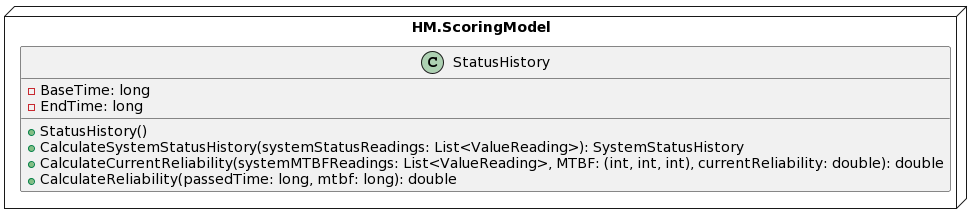
\includegraphics[width=1\textwidth]{StatusHistory.png}
        \caption{Wrapperklasse zur Berechnung von Reliability und der Systemstatus Historie}
        \label{fig:SystemHistoryWrapper}
    \end{figure}
\end{center}
\vspace{-0.5cm}
